%============================================================================%
%
%
%	DOCUMENMT DEFINITION
%
%
%============================================================================%

% we use report class for thesis design
% 11pt font is way bettern to read than 12pt
% we want to make a title page
% two side allows us to make the page layout align by even and odd
% openright tells the compiler that the first page is a right page
\documentclass[pdftex,11pt,titlepage,twoside,openright]{report}	


%----------------------------------------------------------------------------------------
%	ENCODING
%----------------------------------------------------------------------------------------

% for suporting multi platform
\usepackage[utf8x]{inputenc} 	

% natbib is what you want for bibliography
\usepackage[square,authoryear]{natbib}


%----------------------------------------------------------------------------------------
%	ALL DECLARATIONS
%----------------------------------------------------------------------------------------

% here are all our declarations 
%----------------------------------------------------------------------------------------
%	COLOR DEFINITIONS
%----------------------------------------------------------------------------------------

% we use the xtended color package
\usepackage[table,usenames,dvipsnames]{xcolor}

% citation reference color
\definecolor{CITATION_COL}{RGB}{121,0,226}

% urls color
\definecolor{SECTION_COL}{RGB}{0, 117,226}

% internal references color
\definecolor{LINK_COL}{rgb}{0,0,0}

% main color
\definecolor{MAIN_COL}{RGB}{0, 117,226}
% code highlight color
\definecolor{CODE_COL}{rgb}{0.8,0.8,0.8}

% some black fallback
\definecolor{DEF_COL}{RGB}{226,109,0}

%----------------------------------------------------------------------------------------
%	REFERENCES URL CITATION STYLES AND SO ON
%----------------------------------------------------------------------------------------

% apply color definitions to hyperref package
\usepackage[colorlinks=true,citecolor=CITATION_COL,urlcolor=SECTION_COL,linkcolor=LINK_COL]{hyperref}

% make urls directly open the browser onclick
\usepackage{url}
\urlstyle{same}


%----------------------------------------------------------------------------------------
%	FONT DEFINITIONS
%----------------------------------------------------------------------------------------

% better typography rendering scheme
\usepackage[protrusion=true,expansion=true]{microtype} 

 % we use the standard Times font
\usepackage{pslatex}

 % required for accented characters
\usepackage[T1]{fontenc}

% change line spacing here, readability 
% benefits from a slight increase by default
\linespread{1.25} 

% allows more font size definitions
\usepackage{moresize}

%----------------------------------------------------------------------------------------
%	GEOMETRY  DEFINITIONS
%----------------------------------------------------------------------------------------

% define page styles using geometry
\usepackage[bottom=3cm,marginparwidth=1.5cm, marginparsep=0.5cm]{geometry}

 %define A4 Paper
\geometry{a4paper}	

% define margins for even and odd pages
\setlength{\oddsidemargin}{15.5pt}
\setlength{\evensidemargin}{15.5pt}

% paragraph indent and skip
\setlength{\parindent}{0mm}
\setlength{\parskip}{1mm }

% short command for colorizing a text as a note
% not used within this thesis anymore
\newcommand{\NOTE}[1]{\textit{\textcolor{DEF_COL}{#1}}}
	%\marginpar{\sffamily \MakeUppercase{\tiny{{#1}}}}


%----------------------------------------------------------------------------------------
%	GRAPHICS  DEFINITIONS
%----------------------------------------------------------------------------------------

% required for including pictures
\usepackage[pdftex]{graphicx}

 % make it possible to include more than one captioned figure/table in a single float 
\usepackage{subfig}

% make it possible to control text
% positioning around figures
\usepackage{wrapfig}

 % for much better looking tables
\usepackage{booktabs}	

% for better arrays (eg matrices) in maths		
\usepackage{array} 


%----------------------------------------------------------------------------------------
%	ENVIRONMENT  DEFINITIONS
%----------------------------------------------------------------------------------------

 % very flexible & customisable lists
%(eg. enumerate/itemize, etc.)				
\usepackage{paralist}				

% adds environment for commenting
% out blocks of text & for better verbatim
\usepackage{verbatim}				

% allows multiple rows to be merged to one row
\usepackage{multirow}

%----------------------------------------------------------------------------------------
% CUSTOM STRUT FOR EMPTY BOXES
%----------------------------------------- -----------------------------------------------

% when boxes become a pain this might help
\newcommand{\mystrut}{\rule[-.3\baselineskip]{0pt}{\baselineskip}}

%----------------------------------------------------------------------------------------
%	HEADER / FOOTER  DEFINITIONS
%----------------------------------------------------------------------------------------

% header definitions package
 % this should be set AFTER setting up the page geometry
\usepackage{fancyhdr}

% we want to shorten the display of the chapter in the header
\renewcommand{\chaptermark}[1]
{
  \markboth{#1}{}
}

% but we want to show extended info of the current section
\renewcommand{\sectionmark}[1]{\markright{\thesection\ #1}}

% we can even manipulate the font family
%\lhead{\sffamily Chapter \thechapter}

% this defines, what content should be displayed in header and footer
% and on which side (left-right) as well as on even and odd pages
\fancyhf[FLE,FRO]{}
\fancyhf[HLE,HRO]{\colorbox{MAIN_COL}{\sffamily\LARGE\textcolor{white}{\thepage}}}
\fancyhf[HRE,HLO]{\sffamily \textcolor{MAIN_COL}{\leftmark}}
\cfoot{}

%override plain page style for plain pages
\fancypagestyle{plain}{ %
  \fancyhf{} % remove everything
  \renewcommand{\headrulewidth}{0pt} % remove lines as well
  \renewcommand{\footrulewidth}{0pt}
  \fancyhf[HLE,HRO]{\colorbox{MAIN_COL}{\sffamily\large\textcolor{white}{\thepage}}}
  \cfoot{}
}

%----------------------------------------------------------------------------------------
%	SECTION TITLE APPEARANCE
%----------------------------------------------------------------------------------------

% we want to customize our section title 
% to make it look more appealing
\usepackage{sectsty}

% for dimensioning and other math stuff
\usepackage{amsmath}

% modify bg colors
\usepackage[some]{background}

% draw custom graphics progammatically
\usepackage{tikz}				
\usetikzlibrary{shapes, backgrounds,mindmap, trees}

% this is our custom section page layout
\newcommand{\SECTBOX}[1]
{
	\begin{tikzpicture}[remember picture,overlay]
 		\path [fill=MAIN_COL] (current page.west)rectangle (current page.north east); 
	\end{tikzpicture}
}

% this is our custom title page layout
\newcommand{\TITLEBOX}
{
	\begin{tikzpicture}[remember picture,overlay]
 		\path [fill=MAIN_COL] (current page.north west) rectangle (25.0,-3.5); 
	\end{tikzpicture}
}


 % (See the fntguide.pdf for font help)
\allsectionsfont{\sffamily\mdseries\upshape}

% for customizing the title page
\usepackage[explicit]{titlesec}

% font and color def for section
\titleformat{\section}{\LARGE\sffamily}{\textcolor{LINK_COL}{\thesection \hspace{12pt} #1}}{0pt}{}

% font and color def for subsection
\titleformat{\subsection}{\large\bf\sffamily}{\textcolor{SECTION_COL}{\thesubsection \hspace{12pt} #1}}{0pt}{}

% note: remove \thesection or \thesubsection to leave out the 
% numbering at the start of the section / subsection headline


%----------------------------------------------------------------------------------------
%	TABLE OF CONTENT APPEARANCE
%----------------------------------------------------------------------------------------

% deprecated
%\usepackage[nottoc,notlof,notlot]{tocbibind} % Put the bibliography in the ToC

% Alter the style of the Table of Contents
%\usepackage[titles,subfigure]{tocloft}

%\renewcommand{\cftsecfont}{\rmfamily\mdseries\upshape}

%\renewcommand{\cftsecpagefont}{\rmfamily\mdseries\upshape} % No bold!

% renames abstract to executive summary
\renewcommand{\abstractname}{Executive Summary} 		


%----------------------------------------------------------------------------------------
%	CUSTOM HRULE
%----------------------------------------------------------------------------------------

% a custom horizontal rule / line
\newcommand{\HRule}{\rule{\linewidth}{0.5mm}}

\newcommand{\ThinHRule}{\textcolor{CODE_COL}{\rule{0.5\linewidth}{0.05mm}}}


%----------------------------------------------------------------------------------------
%	ENVIRONMENTS
%----------------------------------------------------------------------------------------

% extended listin options
% can be used for code display
\usepackage{listings}

% syntax highlight def for listings
\lstset{ %
  	backgroundcolor=\color{CODE_COL},
	language=C,
	breaklines=true
}

% allows us to define pseudocode algorithms
\usepackage[ruled,linesnumbered]{algorithm2e}

% extended table definitions
\usepackage{tabularx}

% include external pdf pages
\usepackage{pdfpages}
\usepackage{float}


%----------------------------------------------------------------------------------------
%	Code Syntax Highlight Formatting
%----------------------------------------------------------------------------------------

\lstset{
  basicstyle=\ttfamily,
  columns=fullflexible,
  showstringspaces=false,
  commentstyle=\color{gray}\upshape
}

\lstdefinelanguage{XML}
{
  morestring=[b]",
  morestring=[s]{>}{<},
  morecomment= [s]{<!}{->},
  stringstyle=\color{black},
  identifierstyle=\color{blue},
  keywordstyle=\color{orange},
  morekeywords={xmlns, pattern,type, cells, count, required} % list your attributes here which may be highlighted
}






%----------------------------------------------------------------------------------------
%	MAKE INDEX AND GLOSSARY
%----------------------------------------------------------------------------------------


\usepackage[style=long,nonumberlist,toc,xindy,acronym,nomain]{glossaries} % nomain, if you define glossaries in a file, and you use \include{INP-00-glossary}
%\loadglsentries[main]{glossary}
% or using \input:
\newacronym{lvm}{LVM}{Logical Volume Manager}
\newglossaryentry{Linux}
{
  name=Linux,
  description={is a generic term referring to the family of Unix-like
               computer operating systems that use the Linux kernel},
  plural=Linuces
}

\makeglossaries
\usepackage{makeidx}
\makeindex



%============================================================================%
%
%	BEGIN DOCUMENT
%
%============================================================================%


\begin{document}

% before the chapters start, we use roman numbering on the pages
\setcounter{page}{1}
\pagenumbering{roman}

% print title
\begin{titlepage}


%TIKZ BACKGROUND
\TITLEBOX

%CONTENT
\begin{center}



\sffamily\textsc{\HUGE{\textcolor{white}{Master Thesis}}}\\[4cm]


% Upper part of the page. The '~' is needed because \\
% only works if a paragraph has started.

\includegraphics[width=0.45\textwidth]{media/unilogo.png}\makebox[1.5cm]{}
\includegraphics[width=0.15\textwidth]{media/faculty.png}~\\[1.5cm]



% Title
\HRule \\[0.4cm]
{
 \huge \bfseries \sffamily Creating a Master Thesis with LaTex  \\[0.4cm] 
}

\HRule \\[0.4cm] 

\normalfont \large \sffamily A Rough Summary with Code Examples\\[2.5cm]


% Author and supervisor
\noindent
\begin{minipage}{0.4\textwidth}
\begin{flushleft} \large
\emph{Supervisors:} \\
Prof. Dr.~Chris Code\\
Prof. Dr.~Peter Program\\
\end{flushleft}
\end{minipage}%
\begin{minipage}{0.4\textwidth}
\begin{flushright} \large
\emph{Author:}\\
Jan  Küster\\
\url{www.jankuester.com}\\
\end{flushright}
\end{minipage}

\vfill


% Bottom of the page
{\large \today}

\vfill



\vfill
\end{center}
\end{titlepage}



%pagestyle after title
\pagestyle{fancy}

% let's print the table of content, 
% the list of figures and the list of tables
\setcounter{tocdepth}{1}
\tableofcontents
\listoffigures
\listoftables

\cleardoublepage

% EXECUTIVE SUMMARY
% here we describe roughly what this work is about

\begin{abstract}

This work is intended for all those, who want to start writing immediately. For those who aim to avoid the procedure, I went through - all night long figuring out what packages to include. Finding the right syntax to make the intended layout to work. Debugging all those micro errors which may appear. Getting the bibliography to work. And then finally include the citations into the newly written text. By providing this 'out of the box' template, I hope to make things easier for you and to make you start your thesis without hesitation. You should focus on the content your work and not on it's layout because this may stop you from starting to write.\\
This work backs all the topics you need, to get started with your thesis immediately. You may just copy some of the code examples here, which is fine. If you want to create a thesis with your own taste of style, you should dig deeper into the functionality of the packages. The packages and features are focused for work in the field of computer science and include tables, pseudo code, syntax highlighting, mathematical equations and more.

\end{abstract}

% Back to arabic numbering

\pagestyle{fancy}

\setcounter{page}{1}
\pagenumbering{arabic}


%============================================================================%
%
%	CHAPTER 1
%
%============================================================================%

\chapter{General Tools and Techniques for Your Master Thesis}

% before the chapter starts, we can write some overview 
% this is good to summarize quickly what this chapter covers
At this point it may be good for the reader to get an overview about this chapter. What does it cover? What is it's purpose in the bigger picture of your thesis? It is like a micro-abstract and it helps your audience to keep on track. This is especially useful, when your thesis is an interdisciplinary work.



\newpage
%================================================================
%
%	Basic Writing and Citing
%
%================================================================
\section{Basic Commands and Writing Topics}


%-------------------------------------------------------------------------------------------
%	Introduction to Writing
%-------------------------------------------------------------------------------------------
\subsection{Introduction to Writing in LaTex}

The text appearance and the thesis layout is sometimes determined by formal requirements. This text, for example is \NOTE{Times} using 11pt size and a slight increase in space between the text lines. There are also requirements for indenting a new paragraph sometimes.\\
As you can see, this template does not indent the new paragraph. However, you can always change this setting in the \NOTE{declarations.tex} file.\\
\ThinHRule

Some faculties require to include all references to external sources in \NOTE{footnotes}.\footnote{ This is a footnote. You can also include citations and many text formatting LaTex commands.}\footnote{ You may also explain background information on a topic, which may be interesting for further reading.}\footnote{ Footnotes also often include weblinks, for example \url{http://www.jankuester.com}}\\
\ThinHRule

You can enumerate or list some points and sketches of a topic using \NOTE{list or enumerattions}:

\begin{enumerate}
	\item Start
	\item Work
	\item Finish
\end{enumerate}


%-------------------------------------------------------------------------------------------
%	Structure of the thesis
%-------------------------------------------------------------------------------------------
\subsection{Structure of the Thesis}

Since the current template is structured into chapters, sections and subsections. This is mainly because a master thesis may easily grow up to 100 pages and in some cases even bigger. Structuring your big parts into \NOTE{chapters} makes it perfect for separating in logical units, such as:

\begin{itemize}
	\item Introduction
	\item Related Work
	\item Research Design
	\item Proceedings and Data Collection
	\item Data Analysis and Evaluation
	\item Discussion and Conclusion
\end{itemize}
\ThinHRule

The next smaller units are \NOTE{sections} which structure a chapter into it's subtopics. Using \NOTE{subsections} allows to cover these topics step by step and keep the reader on track with a mental model of all the parts of the current topic.\\
\ThinHRule

Now there are also \NOTE{subsubsections} available in LaTex. It would become very confusing when even \NOTE{including subsubsections in the table of contents (toc)}. For this reason, the toc is set to remove these subsubsections. You may alter this by taking a look into the main.tex and the declaration.tex. 
\ThinHRule

\subsubsection{\textcolor{SECTION_COL}{This Subsubsection is not listed in the Table of Contents}}

The advantage is, that your work becomes more structured along the complexity of your topic. It may occur, that topics can become very granular, which is why this is the perfect counterpart for this issue.



%-------------------------------------------------------------------------------------------
%	Using a shorthand command
%-------------------------------------------------------------------------------------------
\subsection{Using a Shorthand Command in Writing}

In the \NOTE{declaration.tex file}, there is a shorthand command called \NOTE{NOTE}. It is created to quickly emphasize important words and let them point out. It is declared by using the \NOTE{newcommand} tag. You may read on the web about this command, since it is very handy once you understand how to use it. You can of course create your own commands but you can also stick to this, if you want to get things done fast.


%-------------------------------------------------------------------------------------------
%	Including citations
%-------------------------------------------------------------------------------------------
\subsection{Including a citation}

Since we use the natbib environment, we need to use citep or citet as commans for our citations. This may look like the following:\\

Standard -  \citep{SkieThea2008} \citep{lombard} \citep{bendavid}\\

With page - \citep[p.123]{BernAnal2010}\\

When the authors, e.g. \citet{mayring2014} said something and you want to embed the citation in your text.

%================================================================
%
%	Basic Writing and Citing
%
%================================================================
\newpage
\section{Including Figures and Tables}


%-------------------------------------------------------------------------------------------
%	Including a graphic
%-------------------------------------------------------------------------------------------
\subsection{Including a Graphic}

Including a graphics is not that hard. Important is to wrap it as a figure, so that it will be included into the \NOTE{ list of figures}. You can also \NOTE{label} it, which allows to refer directly to this figure without the need of keeping track of it's id or name. Another handy parameter is the \NOTE{width} parameter, which allows to set the dimensions according to the current text width.

\begin{figure}[H]
\begin{center}
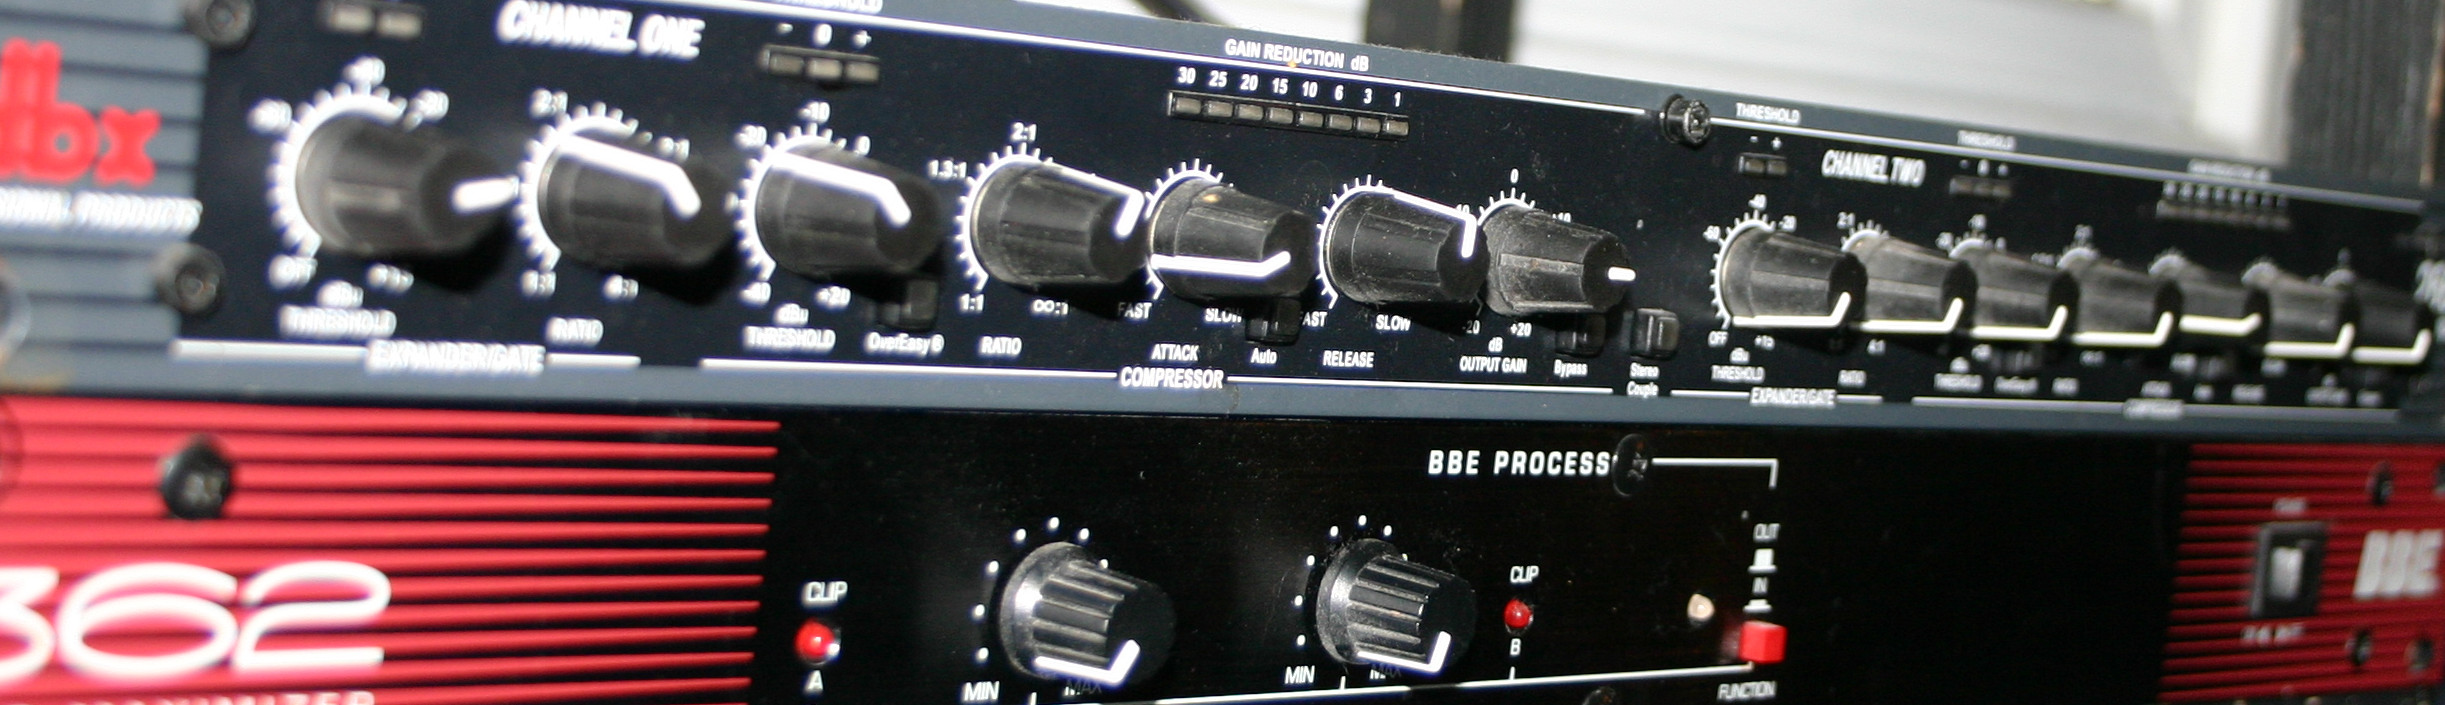
\includegraphics[width=0.8\textwidth]{media/amp.jpg}
\end{center}
\caption[Figure description for the table of content.]{This is the description of the figure. You may even include citations here, which is often important for a master thesis. For example: \citep{SkieThea2008}}
\end{figure}


%-------------------------------------------------------------------------------------------
%	Including a Table
%-------------------------------------------------------------------------------------------
\newpage
\subsection{Including a Table}

When declaring a table, you have multiple options to project complex structures. The following example uses \NOTE{multirows and multicolums} to create a multi-faceted overview of complex data. If you want the table to be listed in the \NOTE{list of tables}, you need to wrap the tabular within a table declaration.

\begin{table}[H]
\begin{tabular}{| l | l | l | l | l |}
\hline
 Category & Levels & \multicolumn{3}{c|}{Scale} \\
&&\multicolumn{3}{c|}{low \hspace*{\fill} high}\\
\hline
 \multirow{5}{*}{A} & 1. first level & low & middle & high \\ \cline{2-5}
 & 2. second level & & & \\ 
 & Subsequence & none & some &many \\
 & Extensions & none & some & all\\ \cline{2-5}
 & 3. presentation & - & text & \cellcolor{green}colored cell \\
\hline
 \multirow{5}{*}{B} & 4. fourth level &  &  &  \\ \cline{2-5}
 & graphics & low & medium & high\\ 
 & sound & mute & normal & loud \\
 & input & mouse & keyboard & gamepad\\ \cline{2-5}
 & 5. fifth leves & Low & Medium & High \\
\hline
\end{tabular}
\caption[Table description for list of tables.]{Detailed description of the table, which can also use various LaTex commands and include citations.}
\end{table}










%============================================================================%
%
%	CHAPTER 2
%
%============================================================================%
\cleardoublepage
\chapter{Specific Tools for a Thesis in Computer Science}

This chapter covers more specific examples, which are useful in the field of computer sciences.

\newpage
\section{Writing Pseudo Code in LaTex}


The package \NOTE{algorithm2e} allows you write nearly all imaginable code structures as pseudo code in LaTex. A referece of commands can be found here: \url{http://www.cs.toronto.edu/~frank/Useful/algorithm2e.pdf}. Do not forget to wrap the pseudo code into a figure, thus it will be included into list of figures.\\

The following example demonstrates the package with a bubble sort algorithm. Note, that the directive \NOTE{repeat - until} is the same as the \NOTE{do-while} directive.

\begin{figure}[H]
\begin{algorithm}[H]
\KwData{A as Array to sort,}
\KwResult{A as sorted Array} 

int n $\leftarrow$ A.size \tcp*[l]{cache the initial size of A}


\Repeat{n>1}{
	int newn $\leftarrow$ 1
	\For{int i=0; i<n-1; i++}
	{
		\If{A[i] > A[i+1]}
		{
			A.swap(i, +1);
		}
	}
	n  $\leftarrow$ newn
}

return A
\caption{bubbleSort(Array A)}
\end{algorithm}
\caption[BubbleSort Algorithm Pseudocoe]{PseudoCode f the BubbleSort Algorithm, derived from \url{https://de.wikipedia.org/wiki/Bubblesort}.}
\end{figure}


\newpage
\section{Mathematical Equations}

Writing mathematical equations can be a very important part of your work. This applies especially, if you want to analyze and evaluate your gathered data. The following example shows a calculation of Kohen's Cappa, a measurement which represents the inter coder reliability in coding qualitative data.\\

Let's assume the following results of coding a text by two different persons:

\begin{table}[H]
\begin{center}
\begin{tabular}{|c|c|c|c|c|c|c|}
\hline
result XY & \multicolumn{6}{c|}{Rater A}\\\hline
 \multirow{6}{*}{Rater B}& & \textbf{9} & \textbf{0} & \textbf{1} & \textbf{2} & \textbf{c(a) }\\\cline{2-7}
 & \textbf{9}& 27	&0&	0	&0 & 0.5510204082\\\cline{2-7}
&\textbf{0}	&0	&6	&0	&0&0.1224489796\\\cline{2-7}
&\textbf{1}	&0	&1	&7	&0&0.1632653061\\\cline{2-7}
&\textbf{2}	&0	&1	&7	&0&0.1632653061\\\cline{2-7}
&\textbf{c(r)} & 0.5510204082 & 0.1632653061 & 0.2857142857 & 0& n=49\\\hline

\end{tabular}
\caption[Example data for mathematical equations]{A set of example data for further use in a mathematical equation.  }
\end{center}
\end{table}

Continuing from this basis, the calculation can be proceeded with Cohen's Kappa defined as

\begin{center}
$k=\frac{Pr(a) - Pr(e)}{1 - Pr(e)}$
\end{center}

Where $Pr(a)$ is the actual observed agreement of the codes and $Pr(e)$ is the estimated agreement of the codes. The actual agreement can be calculated by building the sum of those codes, which have been assigned by both raters (in the table: diagonal from upper left to lower right). This sum is then divided by the amount of responses (n), which is expressed by the following calculation as 

\begin{center}
$Pr(a) = ( 27 + 6 + 7 + 0 ) / 49 = 0.8163265306$
\end{center}

The estimated agreement is calculated out of the percentages of each code in relation to the amount of responses (n). The overall estimated agreement is then built by multiplying these chances and summing up their results. The term is described as

\begin{center}
$Pr(e) = \displaystyle\sum_{i=1}^{m} c(r)_i \times c(a)_i $
\end{center}

where m is the number of all occurring codes, i is the current code and c(r) and c(a) are the chances of assigned codes (see table) for raters and auto. Applying this term is leading to:


\begin{center}
$Pr(e) =  (0.5510204082 \times 0.5510204082) + (0,1632653061 \times 0.1224489796) + (0.285714285 \times 0.1632653061) + (0 \times 0) = 0.3702623907$
\end{center}

The values for Pr(a) and Pr(e) are calculated and can be included into the kappa equation, resulting in the following kappa for item a2s1i1a:

\begin{center}
 $k=\frac{0.8163265306 -0.3702623907}{1 - 0.3702623907} = 0.7083333333$
\end{center}


\section{Including Code into Your Text}

Sometimes you want to include text which include characters that could trigger commands. At this point it useful to wrap them into the \NOTE{verbatim} environment. The text is uninterpreted and listet as is.

\scriptsize
\begin{verbatim}
2015_5_13/23-19-33:550: ************* LOG INFO  *************
2015_5_13/23-19-33:550: name: user1
2015_5_13/23-19-33:550: [0]: 534
2015_5_13/23-19-33:550: [1]: 321
2015_5_13/23-19-33:550: [2]: 094832
2015_5_13/23-19-33:550: [3]: 3980429804
\end{verbatim}
\normalsize	


You can also include existing code and highlight it's syntax, using the \NOTE{lstlisting} package. Look at the declarations.tex file for listings settings. The following example highlights xml syntax by given keywords.

\small
\begin{lstlisting}[keywordstyle=\color{blue},language=XML]
<!-- an XML comment -->
<entry type="normal" pattern="a" />
<entry type="normal" pattern="b" />
<entry type="formula" pattern="t=a+b+c" required="1"/>
\end{lstlisting}
\normalsize	



%============================================================================%
%
%	BIBLIOGRAPHY
%
%============================================================================%

\cleardoublepage
\phantomsection %hyperref package support
\addcontentsline{toc}{chapter}{Bibliography} % add entry to table of contents
\pagestyle{plain}


%{\textbf{\LARGE{Bibliography}}}\\	%headline
%\nocitep{*} % Show all Bib-entries (DEBUG)

\bibliographystyle{abbrvnat}
\bibliography{bib/algorithm.bib,bib/resDes.bib} % for a better structure you can split your bib items into seperate files



\end{document}